\documentclass[11pt, oneside]{article}   	% use "amsart" instead of "article" for AMSLaTeX format


%\usepackage{draftwatermark}
% \SetWatermarkText{Confidential}
% \SetWatermarkScale{5}
% \SetWatermarkLightness {0.85} 
% \SetWatermarkColor[rgb]{0.7,0,0}


\usepackage{geometry}                		% See geometry.pdf to learn the layout options. There are lots.
\geometry{letterpaper}                   		% ... or a4paper or a5paper or ... 
%\geometry{landscape}                		% Activate for for rotated page geometryA. G. Barto, R. S. Sutton, and C. W. Anderson
%\usepackage[parfill]{parskip}    		% Activate to begin paragraphs with an empty line rather than an indent
\usepackage{graphicx}				% Use pdf, png, jpg, or eps� with pdflatex; use eps in DVI mode
								% TeX will automatically convert eps --> pdf in pdflatex		
\usepackage{amssymb}
\usepackage{mathrsfs}
\usepackage{hyperref}
\usepackage{url}
\usepackage{authblk}
\usepackage{amsmath}
\usepackage{mathtools}
\usepackage{graphicx}
\usepackage{fixltx2e}
\usepackage{hyperref}
\usepackage{alltt}
\usepackage{color}
\usepackage{stix}
\usepackage{caption}


\newcommand{\argmax}{\operatornamewithlimits{argmax}}
\newcommand{\argmin}{\operatornamewithlimits{argmin}}
\newcommand\independent{\protect\mathpalette{\protect\independenT}{\perp}}
\def\independenT#1#2{\mathrel{\rlap{$#1#2$}\mkern2mu{#1#2}}}
\DeclareMathOperator{\E}{\mathbb{E}}
\newcommand{\Var}{\mathrm{Var}}
\newcommand{\Cov}{\mathrm{Cov}}



\title{Causal Graphs and Sources of  Bias}
\author{David Meyer \\ dmm@\{1-4-5.net,uoregon.edu,...\}}

\date{Last update: \today}							% Activate to display a given date or no date


\begin{document}
\maketitle


\section{Introduction} 
\label{sec:intro}
Inferring the causal structure of a set of random variables from a finite sample of the joint distribution is an important problem in science.
One way to think about causal structure is that when we observe the world, we are really observing some joint distribution
$P(X_1, \hdots, X_n)$. However, we don't really know which of the $X_i$'s are "causes" and which are "effects" other than that some set of the $X_i$'s is the effected variable $Y$;
the $X_i$'s are sometimes called "treatment variables" and $Y$ is called the "response variable". 

\bigskip
\noindent
Unfortunately these cause/effect relationships aren't represented in non-interventional data. To understand these relationships we need what is called
a Markov (or causal) graph. A graph $G$ is called Markov if it is a DAG and for a given node in the graph, that node is conditionally independent of its non-descendants 
given its parents. That is, $x_j \independent nd_j \mid  pa_j$, where $nd_j$ are the non-descendants of $x_j$ in $G$ 
and $pa_j$ are the parents of $x_j$ in $G$. Said another way,  the joint distribution $p(x_1,\hdots,x_n)$ factorizes: 

\begin{equation*}
p(x_1,\hdots,x_n) = \prod\limits_{j=1}^n p(x_j \mid pa_j) 
\end{equation*}

\bigskip
\noindent
The semantics are that the parents $pa_j$ of $x_j$ in $G$ are $x_j$'s direct causes.  


\bigskip
\noindent
A perhaps more abstract way to think about the Markov condition is that given all the direct causes of an observable $O,$ its non-effects provide 
no additional information on $O$ \cite{Peters:2014:CDC:2627435.2670315}.
The underlying idea here is that "nature chooses" the conditional distributions $p(x_j \mid pa_j)$ independently from one 
another, since the generation of additional independencies (that is, independencies are not imposed by the 
structure of the DAG) would require tuning between these conditional distributions \cite{Peters:2014:CDC:2627435.2670315}.

\bigskip
\noindent
If we do have a such a graph $G$,  can we say anything about the associations (statistical relationships) implied by $G$?
We might think about these associations, that is, the statistical relationships that we observe, more as a bundle of different kinds of associations, 
some of which may be causal and others which are spurious (non-causal). The goal of \emph{causal identification} is to 
eliminate all the non-causal associations (which turn out to  be paths in $G$), leaving only the causal relationships, if any. Figure \ref{fig:associations}
is a cartoon of this situation.


\begin{figure}[h!]
\center{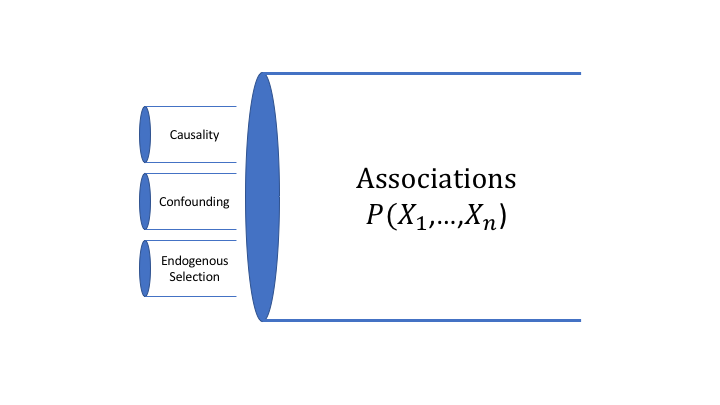
\includegraphics[scale=0.35] {images/associations.png}}
\caption{Associations, joint distributions, and bais}
\label{fig:associations}
\end{figure}

\section{Causality}
 Causality in a Markov graph is represented by a chain structure in which all the arrows are pointing in the same direction (the direction of "time"); 
 this is shown in Figure \ref{fig:direct}. A bit of notation: Two real-valued random variables $A$ and $B$ are said to be \emph{conditionally independent}
 given $C$, written $A \independent B \mid C$, if $\forall A,B$ $P(A, B \mid C) = P(A \mid C) \, P(B \mid C)$ and for $\forall C \, P(C) > 0$. Note that conditional 
 independence neither implies nor is implied by independence. That is,  there are $A,B$ and $C$ such that we have only independence or only conditional independence.
 
\bigskip
\noindent
In our example, we have  $A \not \Vbar B$ and $A \Vbar B \mid C$, that is, $A$ is not independent of $B$ (because $A$ causes $B$),
but conditioning\footnote{Conditioning can be as simple as marginalizing out $C$.}  on $C$ renders $A$ independent of $B$.  
This is called \emph{Overselection Bias} because you conditioned on a node in the chain, resulting in independence ($A \Vbar B \mid C$) when 
in reality $A$ and $B$ are causally related ($A \not \Vbar B$). The solution to Overslection Bias
is not to condition on a node in the chain (here $C$).

\begin{figure}[b!]
\center{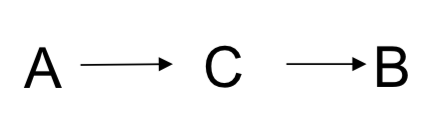
\includegraphics[scale=0.5] {images/direct.png}}
\caption{Causality (chain): $A \not \Vbar B$ and $A \Vbar B \mid C$}
\label{fig:direct}
\end{figure}


\section{Confounding}

A  \emph{confounder} is a (possibly hidden) common cause in a Markov graph. This is shown in Figure \ref{fig:confounding}. The basic idea
here is that there is non-causal path in the graph that is transmitting an association. Here $A$ seems to be causally related to  $B$ ($A \not \Vbar B$) due
to this association.  However, if we remove the non-causal path by conditioning on the confounder $C$, we see that $A$ doesn't really cause  
$B$ ($A \Vbar B \mid C$).  This bias is called \emph{Confounding Bias} or 
sometimes just Confounding.  A  general solution to Confounding is to condition on the common cause ($C$).  Essentially Confounding bias arises from
the failure to condition on a common cause.

\bigskip
\noindent
One of the most famous examples of confounding involves the eminent statistician R.A. Fisher, who claimed (among other things) that the presence of a 
confounder meant that one couldn't conclude that there was a causal link between smoking and lung cancer \cite{FISHER1958}. This is shown in 
Figure \ref{fig:fisher}.

\begin{figure}
\center{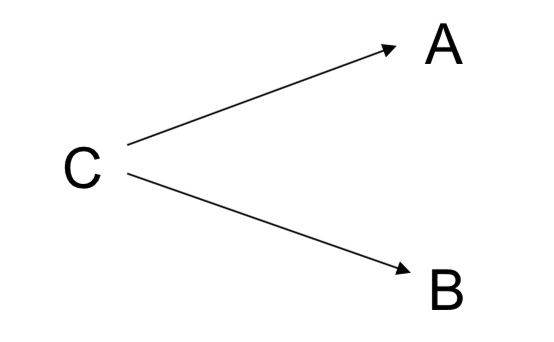
\includegraphics[scale=0.5] {images/confounding.png}}
\caption{Confounding (common cause): $A \not \Vbar B$ and $A \Vbar B \mid C$}
\label{fig:confounding}
\end{figure}

 
 
\begin{figure}[b]
\center{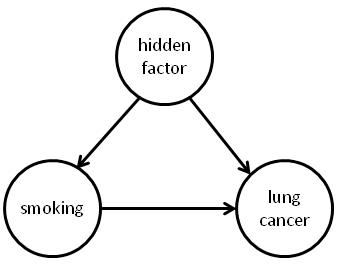
\includegraphics[scale=0.7] {images/smoking_basic_causal_model.png}}
\caption{R. A. Fisher, smoking, lung cancer and confounding}
\label{fig:fisher}
\end{figure}

\section{Endogenous Selection}

The structure of the graph representing Endogenous Selection is shown in Figure \ref{fig:collider}.  You can see how \emph{Endogenous Selection Bias}
comes about in the following classic example \cite{doi:10.1146/annurev-soc-071913-043455}:  Consider the following causal model for the 
relationships between productivity, $A$, originality, $B$, 
and academic tenure, $C$. $C$ here is called a "collider". 
Now, suppose that productivity and originality are unassociated in the general population (i.e., productivity does not cause originality and originality does 
not cause productivity (i.e. $A \independent B$), and productivity and originality do not share any common cause). 
Suppose further that originality and productivity are separately sufficient for promotion to tenure.  In this case, tenure is a collider variable. 


\begin{figure}
\center{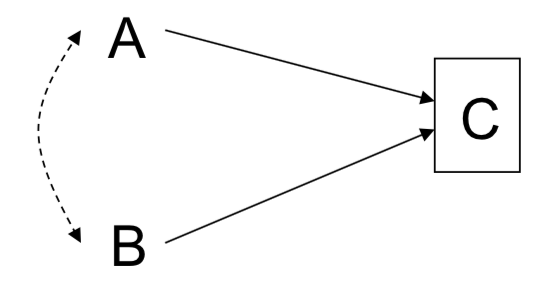
\includegraphics[scale=0.5] {images/collider.png}}
\caption{Endogenous Selection (common outcome): $A \Vbar B$ and $A \not \Vbar B \mid C$}
\label{fig:collider}
\end{figure}

\bigskip
\noindent
Now if you condition on tenure (the collider, C) then you are assessing the relationship between originality and productivity only among tenured faculty (showing 
that Endogenous Selection Bias subsumes Sample Selection Bias \cite{2008arXiv0805.2775C}). In this case knowing that an unoriginal scholar has tenure implies 
that he must have been productive. Conversely, knowing that an unproductive scholar has tenure implies that he must have been original. In either case conditioning 
on the collider tenure (C) creates an association between productivity (A) and originality (B) among  tenured faculty, even though one does not cause the other. This form 
of bias is called \emph{Endogenous Selection Bias} and is closely related to Berkson's paradox \cite{Westreich2012} and "explaining away"  \cite{Wellman:1993:EEA:628299.628453}.

\bigskip
\noindent
Perhaps surprisingly, in Endogenous Selection Bias $A$ and $B$ are independent ($A$ and $B$ don't cause one another, $A \Vbar B$), but conditioning on (knowing) $C$ induces a 
relationship between $A$ and $B$ that doesn't exist in the population. That is, $A \not \Vbar B \mid C$. The solution here is not to condition on a 
collider (or any node downstream of the collider). Endogenous selection bias results from the mistaken conditioning on a common effect.

\section{d-separation}
Finally, can you read any of these relationships directly off the graph? In certain situations the answer is yes. The rule we use for this, called \emph{d-separation}, is due
to Pearl \cite{Pearl:1988:PRI:52121}. Pearl describes d-separation as a "gift from the gods" since it allows us to deduce properties of the statistical distribution (associations) 
from the causal  graph. Of course, in order to do this, you need the causal graph. So where does the causal graph come from? That is a whole different issue, but suffice it to 
say that nature doesn't reveal causal structure in non-interventional data, so we have to get it somewhere else. Discovering the causal graph (or other representation) is called 
\emph{causal discovery}.  In causal discovery (also called structure learning) we're trying to reconstruct the structural causal model or its graphical representation from its joint 
distribution $p(X_1, \hdots, X_n)$.

\bigskip
\noindent
In general, we would like to ask the question:  Under what 
assumptions on the data generating process can one infer the causal graph from the joint distribution? There is pretty vast literature here. One place to start might be 
\cite{Peters:2011:ICG:3020548.3020617}. 


\newpage
\bibliographystyle{ieeetr}
\bibliography{/Users/dmm/papers/bib/ml}



\end{document} 
